\section{Shared Memory Programming Model}

In this section, the performance of MPI$_{sm}$ and OpenMP is directly compared in the context of the shared memory programming model. The objective of this comparison is to test the capabilities of MPI$_{sm}$ and to evaluate its viability as an alternative to OpenMP in this programming model.

\medskip

A simple algorithm implementing a three point stencil, similar to the one used to numerically evaluate a second derivative, is used for this purpose. The algorithm is shown in Figure \ref{fig:ThreePointStencil}.

\medskip
  
\begin{figure} [h!]
\centering
\captionsetup{justification=centering, singlelinecheck=false}
\begin{lstlisting}[style=CStyle]
for(int i = start; i < end; ++i) {
    derivative[i] =  0.25*(fun[i+1] + fun[i-1] - 2.0 * fun[i]);
} // end for //
\end{lstlisting}    
\caption{Three point stencil.}
\label{fig:ThreePointStencil}
\end{figure}

\begin{comment}
\begin{figure} [h!]
\centering
\captionsetup{justification=centering, singlelinecheck=false}
\begin{lstlisting}[style=CStyle]
for(int l = start; l < end; ++l) {
    for(int r = 1; r < ydim ; ++r) {
        for(int c = 1; c < xdim; ++c) {
            int k = c + r*COL2 + l*COL2*ROW2;
            derivative[k] =  0.25*(fun[k+1] + fun[k-1] - 2.0 * fun[k]);
        } // end for //
    } // end for //
} // end for //
\end{lstlisting}    
\caption{Three point stencil.}
\label{fig:ThreePointStencil}
\end{figure}
\end{comment}


\medskip

Results from two versions of the program (MPI$_{sm}$ and OpenMP), produced by three compilers, are compared discussed below.

\subsection*{Preliminary Result}

Figure \ref{fig:sharedMemoryProgrammingModel} presents results obtained on \textbf{stout}. Results on other systems show the same general behavior. The plot on the left (\ref{fig:sharedMemoryComparison}) shows actual execution time while the right plot (\ref{fig:sharedMemoryRatioComparison}) presents the ratio between the time taken by the OpenMP to the MPI$_{sm}$ version of this program, as a function of the number of threads/processors used. Notice that this ratio is the opposite of the one used in Figures \ref{fig:TriadRatioBefore} and \ref{fig:TriadRatio}. In every instance, the ratios were selected in such a way that any value greater than one means that MPI$_{sm}$ performs better than OpenMP.

\medskip

In Figure \ref{fig:sharedMemoryComparison} the segmented lines correspond to OpenMP while the continuous lines represent MPI$_{sm}$. This figure clearly shows that, in general, the OpenMP version (segmented lines) outperforms the MPI$_{sm}$ version when more than one thread/process are used in the solution. Figure \ref{fig:sharedMemoryRatioComparison} permits a better assessment of the problem by showing how the relative performance of MPI$_{sm}$ clearly deteriorates with respect to OpenMP as more processes are incorporated.


\medskip

Given the results of the stream benchmark and of the barriers comparison obtained in section \ref{potentialLimits}, this was an unexpected and disappointing result.

\begin{figure} [h!]
    \centering
    \captionsetup{justification=centering, singlelinecheck=false}
    \begin{subfigure}{.6\textwidth}
      \centering
      \hspace*{-1.5cm} 
      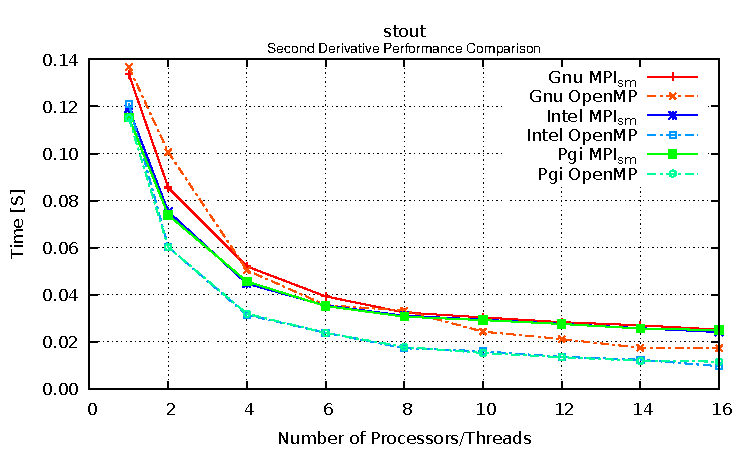
\includegraphics[width=0.95\linewidth]{Plots/SMPM/stoutShowingEffectOfFirstTouch.pdf}
      \caption[]{Estimated time.}
      \label{fig:sharedMemoryComparison}
    \end{subfigure}%
    \begin{subfigure}{.6\textwidth}
      \centering
      \hspace*{-1.5cm} 
      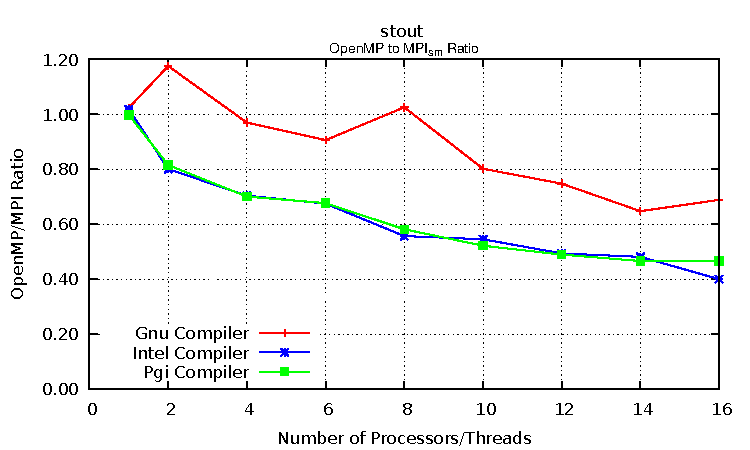
\includegraphics[width=0.95\linewidth]{Plots/SMPM/stoutRatioShowingEffectOfFirstTouch.pdf}
      \caption{OpenMP to MPI$_{sm}$ Ratio.}
      \label{fig:sharedMemoryRatioComparison}
    \end{subfigure}%
\caption{Shared Memory Programming Model Comparison - Faulty case.}
\label{fig:sharedMemoryProgrammingModel}
\end{figure}


\subsection*{First Touch Policy}

Exploring the possible causes of the behavior shown in Figure \ref{fig:sharedMemoryProgrammingModel}, an important  difference between the OpenMP and the MPI$_{sm}$ implementation of the algorithm was discovered: while in the OpenMP version, the arrays were initialized in parallel, in the MPI$_{sm}$ version a single process was in charged of the initialization. This apparently simple difference trigger a well known problem in ccNuma systems, \textbf{page placement by first touch}. 

\medskip

Page placement by first touch is a well known policy in which a memory page gets mapped into the locality domain (socket) of the processor that first writes to it. Processors usually performs better when memory is directly attached to the socket that they are on. Any access to memory from another socket has additional latency overhead compared to accessing local memory. Therefore, remote memory accesses should be to avoided if possible. Proper placement of data will increase the overall bandwidth and improve the latency to memory.

\medskip

To initialize the array using a single process in the MPI$_{sm}$ version was a conceptual error. However, we decided to show the faulty results (Figure \ref{fig:sharedMemoryProgrammingModel}) to remark, on the one hand, the consequences of that error, and, on the other hand, to show that it can also happen with MPI$_{sm}$.

\subsection*{Corrected Result}

Once the cause of the performance deterioration in the MPI$_{sm}$ version was identified and corrected, the programs were run again and the results are shown in Figure \ref{fig:sharedMemoryProgrammingModel2}.

\medskip

A comparison between Figures \ref{fig:sharedMemoryProgrammingModel} and \ref{fig:sharedMemoryProgrammingModel2} clearly shows the performance improvement of the MPI$_{sm}$ version relative to its OpenMP counterpart after correcting for the \emph{first touch} policy. 

\medskip

Figure \ref{fig:sharedMemoryRatioComparison2} shows that the relative performance of the two versions is about the same for programs produced by the Intel and PGI compilers. For the GNU compiler, the MPI$_{sm}$ version outperforms the OpenMP version. However, this superior behavior of MPI$_{sm}$ version produced by the GNU compiler did not occur in all the systems tested. For example, the results obtained on a different system, \textbf{koelsch}, presented in Figure \ref{fig:sharedMemoryProgrammingModel3}, shows an even performance of MPI$_{sm}$ and OpenMP in all the tested compilers.


\begin{figure} [t!]
    \centering
    \captionsetup{justification=centering, singlelinecheck=false}
    \begin{subfigure}{.6\textwidth}
      \centering
      \hspace*{-1.5cm} 
      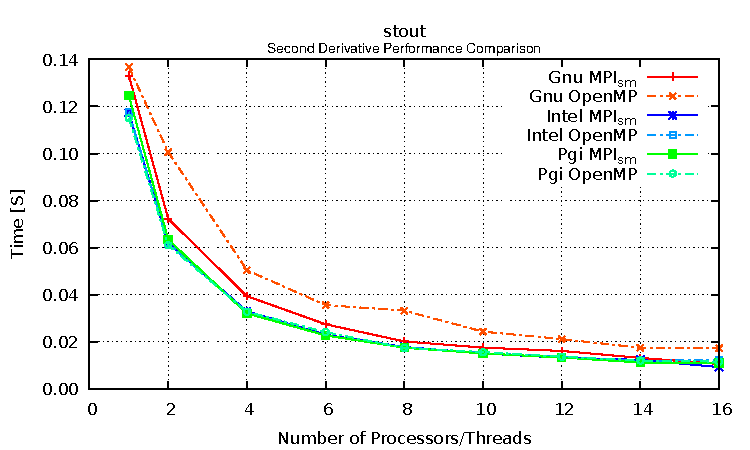
\includegraphics[width=0.95\linewidth]{Plots/SMPM/stout.pdf}
      \caption[]{Estimated time.}
      \label{fig:sharedMemoryComparison2}
    \end{subfigure}%
    \begin{subfigure}{.6\textwidth}
      \centering
      \hspace*{-1.5cm} 
      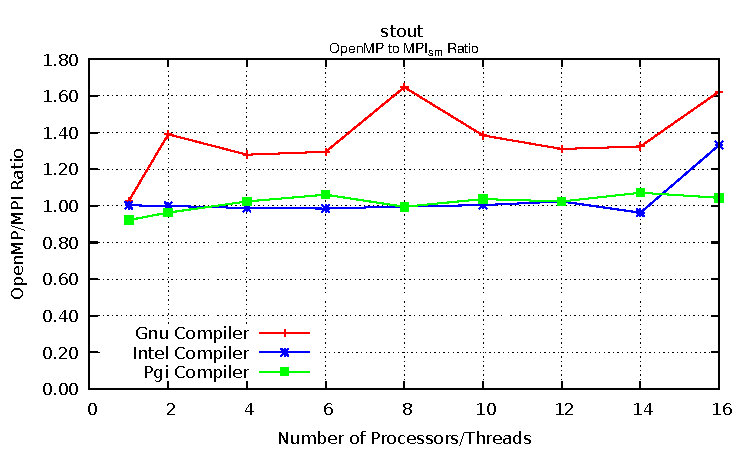
\includegraphics[width=0.95\linewidth]{Plots/SMPM/stoutRatio.pdf}
      \caption{OpenMP to MPI$_{sm}$ Ratio.}
      \label{fig:sharedMemoryRatioComparison2}
    \end{subfigure}%
\caption{Shared Memory Programming Model Comparison.}
\label{fig:sharedMemoryProgrammingModel2}
\end{figure}



\begin{figure} [t!]
    \centering
    \captionsetup{justification=centering, singlelinecheck=false}
    \begin{subfigure}{.6\textwidth}
      \centering
      \hspace*{-1.5cm} 
      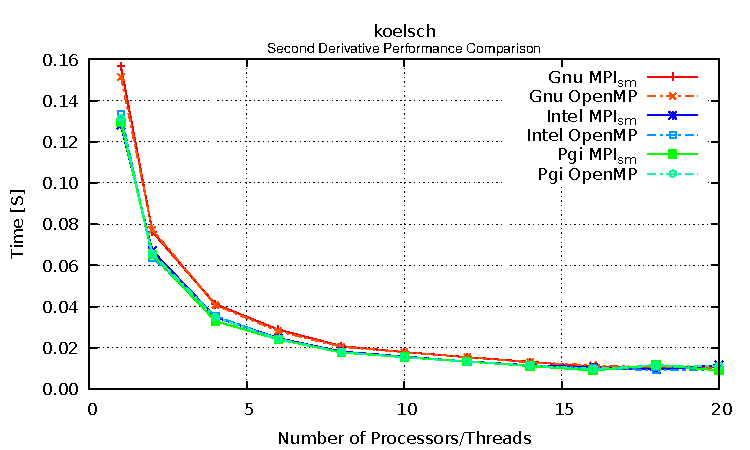
\includegraphics[width=0.95\linewidth]{Plots/SMPM/koelsch.pdf}
      \caption[]{Estimated time.}
      \label{fig:sharedMemoryComparison3}
    \end{subfigure}%
    \begin{subfigure}{.6\textwidth}
      \centering
      \hspace*{-1.5cm} 
      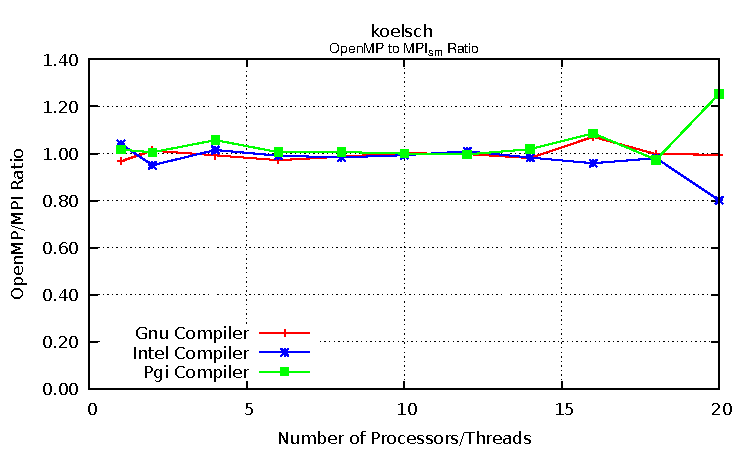
\includegraphics[width=0.95\linewidth]{Plots/SMPM/koelschRatio.pdf}
      \caption{OpenMP to MPI$_{sm}$ Ratio.}
      \label{fig:sharedMemoryRatioComparison3}
    \end{subfigure}%
\caption{Shared Memory Programming Model Comparison.}
\label{fig:sharedMemoryProgrammingModel3}
\end{figure}


\medskip

\subsection*{Summary}

In this section, a comparison of the performance of two shared memory programming paradigms, OpenMP and MPI$_{sm}$, was discussed. The performance was associated with the time required to execute a simple algorithm. The results obtained lead to conclude that the achievable performance of these two shared memory programming models is essentially the same. This implies that the decision to choose between them should not be based on pure performance.



%using of OpenMP and MPI$_{sm}$ in the  is similar.
